\section{Constraints}
\subsection{``.xdc''-Dateien}
Physikalische Eigenschaften eines Designs können dem Synthese- und Implementierungstool mit Constraints mitgeteilt werden. Diese Constraints werden bei Vivado in ``.xdc''-Dateien definiert. Sind mehrere Dateien vorhanden, so werden diese sequentiell angewendet. Wird ein Constraint mehrfach gesetzt, so wird der zuletzt gesetzte Constraint verwendet. Für jede ``.xdc''-Datei kann desweiteren definiert werden, ob sie nur in der Synthese oder nur der Implementation angewendet werden soll (oder bei beidem).
\lstinputlisting[language=tcl]{code/tcl/xdc_property_used_in.xdc}

\subsubsection{Reihenfolge}
Es wird empfohlen die Constraints in der nachfolgenden Reihenfolge in den Dateien abzulegen, um Fehler zu minimieren.
\begin{multicols}{3}
    \begin{compactenum}
        \item Timing Assertions
        \begin{compactenum}
            \item Primary Clocks
            \item Virtual Clocks
            \item Generated Clocks
            \item Clock Groups
            \item Input und Output Delay
        \end{compactenum}
        \item Timing Exceptions
        \begin{compactenum}
            \item False Paths
            \item Max Delay / Min Delay
            \item Multicycle Paths
            \item Case Analysis
            \item Disable Timing
        \end{compactenum}
        \item Physical Constraints \\ \ \\ \ \\ \ \\
    \end{compactenum}
\end{multicols}

\subsection{Timing Analysis}
Um Constraints bestimmen zu können, muss als erstes eine Timing Analyse durchgeführt werden. Eine Timing Analyse soll sicherstellen, dass alle Timing Anforderungen aller Komponenten eingehalten werden. \\
\begin{minipage}{0.65\textwidth}
    \begin{figure}[H]
        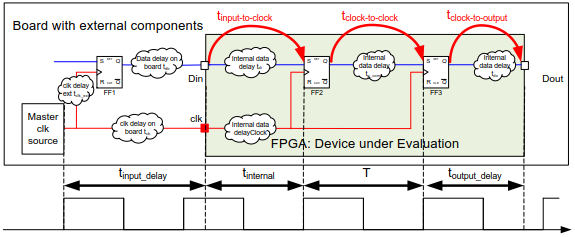
\includegraphics[width=\textwidth]{images/static_timing_analysis.png}
    \end{figure}
\end{minipage}
\hfill
\begin{minipage}{0.3\textwidth}
    Eine statische Timing Analyse muss die nachfolgenden Situationen abdecken:
    \begin{compactitem}
        \item Clock-to-Clock Pfad
        \item Input-to-Clock Pfad
        \item Clock-to-Output Pfad
    \end{compactitem}
    \ \\ \ \\ \ \\ \ \\ \ \\
\end{minipage}
\hspace*{+1cm}
\begin{multicols}{2}
    \subsubsection{Input Delay}
    Das Input Delay kann mit der nachfolgenden Formel bestimmt werden, weiterführende Informationen sind in Kapitel \ref{chapter:input_delay} zu finden. \\
    $t_{\text{input\_delay}}=t_{\text{clk\_ext}}+t_{\text{pcq\_FF1}}+t_{\text{db}}-t_{\text{cb}}$

    \subsubsection{Output Delay}
    Das Output Delay kann mit der nachfolgenden Formel bestimmt werden, weiterführende Informationen sind in Kapitel \ref{chapter:output_delay} zu finden. \\
    $t_{\text{output\_delay}}=t_{\text{pcq\_FF3}}+t_{\text{p\_comb}}+t_{\text{clk\_latency(FF3-master)}}$
\end{multicols}

\begin{multicols}{2}
    \subsubsection{Clock Skew}
    Der Skew ist die Timing Differenz zwischen zwei Signalen. Der Clock Skew ist die Differenz zwischen zwei Clock Signalen. Dieser Clock Skew sollte im Idealfall immer 0 sein. Da dies aber nicht realisierbar ist, implementieren die Synthesetools Clock Trees um den Clock Skew zu minimieren. Typischerweise ist der Clock Skew somit im Bereich von ps bis ns.
    \ \\ \ \\
    \begin{figure}[H]
        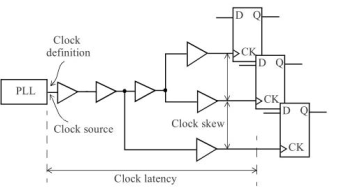
\includegraphics[width=0.35\textwidth]{images/clock_skew.png}
    \end{figure}
\end{multicols}

\subsubsection{Slack}
Der Slack bezeichnet die Differenz zwischen der benötigten Ankunftszeit eines Signales und der tatsächlichen Ankunftszeit. Solange der Slack einen positiven Wert aufweist, ist das Timing korrekt. Wird der Slack negativ, so können Timinganforderungen nicht mehr eingehalten werden.

\paragraph{Berechnung}
\begin{minipage}{0.3\textwidth}
    \begin{figure}[H]
        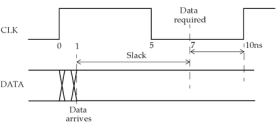
\includegraphics[width=1\textwidth]{images/slack.png}
    \end{figure}
\end{minipage}
\hfill
\begin{minipage}{0.65\textwidth}
    $Slack=RequiredTime-ArrivalTime$ wobei $RequiredTime=Tperiod-Tsetup(CaptureFlipFlop)$ \\
    Nach nebenstehendem Bild: $RequiredTime=10ns-3ns=7ns$ und $ArrivalTime=1ns$ ergibt $Slack=7ns-1ns=6ns$
\end{minipage}

\subsection{Clocks}
Clocks müssen definiert werden, damit die Timing Paths berechnet werden können. Ein Clock wird dabei so definiert, wie er am Startpunkt des Clock Trees aussieht (in der Regel der Eingangspin des Clocks). Es wird angegeben, wie gross die Periode des Clocks ist, sowie wo die Flanken sind. Alle Zeiten werden dabei in Nanosekunden angegeben.

\subsubsection{Primary Clocks}
Ein Primary Clock ist ein Clock, welcher in der Regel durch einen Eingangspin zugeführt wird. Ein solcher Clock muss immer einem Netzlistenobjekt zugewiesen werden. \\
Der nachfolgende Befehl definiert einen neuen Clock mit dem Namen \textit{devclk}, einer Periode von 10ns sowie einem Dutycycle von 25\%. Der Clock wird über den Port \textit{clkin} zugeführt.
\lstinputlisting[language=tcl]{code/tcl/primary_clock.xdc}

\subsubsection{Generated Clocks}
Generated Clock werden von speziellen Blöcken in einem FPGA generiert (z.B. MMCM). Sie können auch von Userlogik erzeugt werden. Diese Generated Clocks sind jedoch an einen anderen Clock gebunden und teilen diesen z.B. herunter, oder bewirken eine Phasenverschiebung.

\subsubsection{Virtual Clocks}
Ein Virtual Clock ist ein Clock welcher physikalisch nicht existiert und somit nicht an ein Netzlisten-Objekt gebunden ist. Sie werden benutzt um Input- und Output-Delays zu spezifizieren, wenn das externe Gerät mit einem anderen Clock läuft als der FPGA. \\
Der nachfolgende Befehl definiert einen neuen Virtual Clock mit dem Namen \textit{virtclk}, einer Periode von 10ns sowie einem Dutycycle von 25\%.
\lstinputlisting[language=tcl]{code/tcl/virtual_clock.xdc}

\subsubsection{Clock Latency}
\begin{minipage}{0.5\textwidth}
    \begin{figure}[H]
        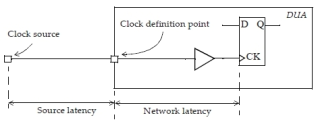
\includegraphics[width=1\textwidth]{images/clock_latency.png}
    \end{figure}
\end{minipage}
\hfill
\begin{minipage}{0.45\textwidth}
    Clocks erreichen verschiedene Punkte in einem Design mit unterschiedlichen Verzögerungen. Diese Verzögerungen können in zwei Arten unterschieden werden:
    \begin{compactitem}
        \item Network Latency
        \item Source Latency
    \end{compactitem} \ \\ \ \\
\end{minipage}

Mit den nachfolgenden Befehlen können die Latenzen definiert werden. Wird nichts spezifisch angegeben, so werden der  \textit{min}, \textit{max}, \textit{rise} und \textit{fall} Wert gesetzt.
\lstinputlisting[language=tcl]{code/tcl/clock_latency.xdc}

\subsubsection{Clock Jitter}
\begin{minipage}{0.3\textwidth}
    \begin{figure}[H]
        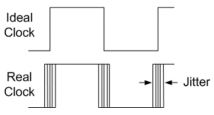
\includegraphics[width=1\textwidth]{images/clock_jitter.png}
    \end{figure}
\end{minipage}
\hfill
\begin{minipage}{0.65\textwidth}
    Aufgrund der physikalischen Eigenschaften ist kein Clock ideal. Kleinere Schwankungen in der Übertragung können auftreten. Diese Schwankungen werden Jitter genannt und in Nanosekunden gemessen. \ \\ \ \\ \ \\
\end{minipage}

\paragraph{Input Jitter}
Input Jitter definiert Jitter auf Primary Clocks. Mit dem nachfolgenden Befehl kann der Jitter definiert werden:
\lstinputlisting[language=tcl]{code/tcl/input_jitter.xdc}

\paragraph{System Jitter}
Der System Jitter spezifiert den Jitter für alle Clocks im System (auch für die Primary Clocks). Er wird benutzt um starkes Rauschen zu modellieren. Mit dem nachfolgenden Befehl kann der Jitter definiert werden:
\lstinputlisting[language=tcl]{code/tcl/system_jitter.xdc}

\begin{multicols}{2}
    \subsubsection{Zusätzliche Clock Unsicherheit}
    Sind weitere Unsicherheiten zwischen verschiedenen Clocks vorhanden, so kann mit dem nachfolgenden Befehl definiert werden, wie sich verschiedene Clocks zueinander verhalten.
    \lstinputlisting[language=tcl]{code/tcl/clock_uncertainty.xdc}
    \begin{figure}[H]
        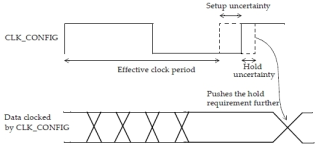
\includegraphics[width=0.5\textwidth]{images/clock_uncertainty.png}
    \end{figure}
\end{multicols}

\subsection{I/O Pin Constraints}
\lstinputlisting[language=tcl]{code/tcl/io_pin_constraints.xdc}

\subsection{I/O Delay}
Damit externe Timing-Anforderungen korrekt in die Synthese und Implementation einbezogen werden können, ist es notwendig diese anzugeben.

\subsubsection{Input Delay} \label{chapter:input_delay}
Input Delays geben an, mit welcher Verzögerung Daten an einem Eingangsport anliegen. Diese Verzögerung muss relativ zu einem Clock angegeben werden.

\paragraph{Tcl Befehl}
Mit dem Befehl \texttt{set\_input\_delay} kann das Input-Delay angegeben werden. Die folgenden Parameter werden dabei unterstützt:
\begin{compactitem}
    \item \texttt{-clock}: Gibt den Clock an, zu welchem die Verzögerung gilt.
    \item \texttt{-min}, \texttt{-max}: Definiert die min Zeit (hold/removal) oder die max Zeit (setup/recovery). Wird dieser Parameter nicht spezifisch angegeben, so wird die Input-Delay-Zeit für min und max verwendet.
    \item \texttt{-clock\_fall}: Gibt an, dass der Input-Delay relativ zur fallenden Clockflanke gilt.
    \item \texttt{-rise}, \texttt{-fall}: Gibt an, für welche Flanke des Eingangssignales die Angaben gelten.
    \item \texttt{-add\_delay}: Diese Option wird benutzt, wenn ein zweites Delay angegeben werden muss (z.B. bei DDR).
\end{compactitem}

\paragraph{Beispiel}
\begin{figure}[H]
    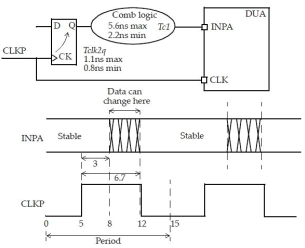
\includegraphics[width=0.5\textwidth]{images/input_delay.png}
\end{figure}
\lstinputlisting[language=tcl]{code/tcl/input_delay.xdc}

\subsubsection{Output Delay} \label{chapter:output_delay}
Output Delays geben an, in welchem Zeitbereich die Daten am Ausgangsport stabil sein müssen. Dieser Zeitbereich wird wiederum relativ zu einem Clock angegeben.

\paragraph{Tcl Befehl}
Mit dem Befehl \texttt{set\_output\_delay} kann das Output-Delay angegeben werden. Die folgenden Parameter werden dabei unterstützt:
\begin{compactitem}
    \item \texttt{-clock}: Gibt den Clock an, zu welchem die Zeit gilt.
    \item \texttt{-min}, \texttt{-max}: Definiert die min Zeit (hold/removal) oder die max Zeit (setup/recovery). Wird dieser Parameter nicht spezifisch angegeben, so wird die Input-Delay-Zeit für min und max verwendet.
    \item \texttt{-clock\_fall}: Gibt an, dass der Output-Delay relativ zur fallenden Clockflanke gilt.
    \item \texttt{-rise}, \texttt{-fall}: Gibt an, für welche Flanke des Ausgangssignales die Angaben gelten.
    \item \texttt{-add\_delay}: Diese Option wird benutzt, wenn ein zweites Delay angegeben werden muss (z.B. bei DDR).
\end{compactitem}

\paragraph{Beispiel}
\begin{figure}[H]
    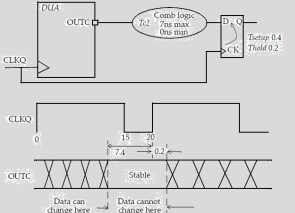
\includegraphics[width=0.5\textwidth]{images/output_delay.png}
\end{figure}
\lstinputlisting[language=tcl]{code/tcl/output_delay.xdc}
